\documentclass[11pt]{article}
\usepackage{geometry, times}                % See geometry.pdf to learn the layout options. There are lots.
\geometry{letterpaper}                   % ... or a4paper or a5paper or ... 
%\geometry{landscape}                % Activate for for rotated page geometry
\usepackage[parfill]{parskip}    % Activate to begin paragraphs with an empty line rather than an indent
\usepackage{fullpage, graphicx, amssymb, epstopdf, hyperref}
\hypersetup{
  colorlinks,
  linkcolor=blue,
  urlcolor=blue
}
\renewcommand{\UrlBreaks}{\do\&\do\=\do\?\do\-\do\/\do\.}
\usepackage{float}
\usepackage{verbatim}
\usepackage{pdfpages}

\DeclareGraphicsRule{.tif}{png}{.png}{`convert #1 `dirname #1`/`basename #1 .tif`.png}


%\VignetteIndexEntry{Using seawaveQ}
\usepackage[utf8]{inputenc}

\title{Vignette for seawaveQ---An R Package Providing a Model and Utilities for Analyzing Trends in Chemical Concentrations in Streams with a Seasonal Wave (seawave) and Adjustment for Streamflow (Q) and Other Ancillary Variables}
\author{Karen R. Ryberg and Aldo V. Vecchia}
\date{\today}                                % Activate to display a given date or no date

\usepackage{Sweave}
\begin{document}
\maketitle
\tableofcontents

\section{Introduction}

This R package, \textbf{seawaveQ}, is designed  for fitting a parametric regression model for assessing variability and trends in pesticide concentration in streams and was developed by Vecchia and others (2008), and subsequently refined and referred to as the ``seawave-Q'' model in several trend analyses (Ryberg and others, 2010; Sullivan and others, 2009; Vecchia and others, 2009).  In these publications, ``seawave-Q'' stands for seasonal wave (seawave) with adjustment for streamflow (Q).  The model was developed to ``handle a number of difficulties often found in pesticide data, such as strong seasonality in response to use patterns, high numbers of concentrations below laboratory reporting levels (RLs), complex relations between streamflow and concentration, and intermittent or changing sampling frequencies (both inter-annually and intra-annually)'' (Vecchia and others, 2008).  This R package provides a standardized methodology for fitting the seawaveQ model and makes the trend analysis method widely available for use by others. In addition, several enhancements to the seawaveQ model have been included as well as utility functions for working with chemical concentration data.  The enhancements and utilities include procedures for preparing and summarizing input data; flexibility to include other explanatory variables besides streamflow; graphical methods for assessing model fit; and plotting routines that may be used for pesticide and other chemical concentration data.  A flow chart showing how the various function in the package work together is shown in figure 1 of the U.S. Geological Survey Open-File Report documenting this package (Ryberg and Vecchia, 2013). 

The statistical methodology for the seawaveQ model is described in Vecchia and others (2008) and in the U.S. Geological Survey Open-File Report documenting this package (Ryberg and Vecchia, 2013).   Users new to this model should read both of those documents before applying the model to their own data.  An important part of the model and the output shown below is the seasonal wave. The seasonal wave is a periodic (period of 1 year) solution to a differential equation (Vecchia and others, 2008) that has a pulse input function, a seasonal shift that determines the time at which the seasonal wave reaches its maximum, and a model half-life (see appendix 3.  Visualizations of the Seasonal Wave; Ryberg and Vecchia, 2013).

\section{Input Data}

The seawaveQ model needs two types of input data.  The first is the the water-quality sample data including dates, the concentration data, and qualification codes, indicating which values are censored (less than a laboratory reporting level).  The second type of data is the continuous ancillary data used in the model, such as streamflow anomalies (Ryberg and Vecchia, 2012).  These ancillary data also are used to produce a continuous estimate of pesticide concentration.  Examples of the necessary format of these two datasets are provided and documented in the package.  The following code shows how to access the example data.
\vspace{5 mm}

\begin{Schunk}
\begin{Sinput}
> options(width=65)
> # load waterData package, assuming it has already been installed on the system
> library(seawaveQ)
> # load example data that comes with the package
> data(swData)
> # show first few rows of water-quality data for Missouri River at Omaha, Nebr.
> head(qwMoRivOmaha)
\end{Sinput}
\begin{Soutput}
     staid      dates times R04035 P04035 R04037 P04037 R04041
1 06610000 1996-01-13  1130      <  0.004      _  0.024      <
2 06610000 1996-02-13  1200      <  0.004      E  0.005      <
3 06610000 1996-03-13  1000      E  0.005      E  0.004      <
4 06610000 1996-03-28  1030      <  0.004      E  0.005      _
5 06610000 1996-04-09  1100      _  0.007      E  0.006      _
6 06610000 1996-04-23  1000      <  0.004      <  0.004      _
  P04041 R39415 P39415 R46342 P46342 R82630 P82630 R82661 P82661
1  0.008      _  0.006      <  0.003      _  0.029      <  0.003
2  0.008      _  0.200      <  0.003      <  0.007      <  0.003
3  0.008      _  0.026      <  0.003      <  0.007      <  0.003
4  0.009      _  0.026      <  0.003      <  0.007      <  0.003
5  0.014      _  0.075      E  0.003      <  0.007      <  0.003
6  0.012      _  0.040      <  0.003      <  0.007      <  0.003
  R82668 P82668
1      _  0.008
2      _  0.007
3      E  0.004
4      _  0.008
5      _  0.009
6      <  0.002
\end{Soutput}
\begin{Sinput}
> # get a description of the data including definitions of the columns
> # by viewing the help documentation
> ?qwMoRivOmaha
\end{Sinput}
\end{Schunk}

Optionally, functions have been provided to plot concentration data.  These functions produce scatter plots and box plots that indicate or take into account the censored, less than, values.  The functions are \textit{cenScatPlot} and \textit{rosBoxPlot} and examples of their use follow.  The box plots are generated using the function \textit{ros}, regression on order statistics, in the R package \textbf{NADA} (Lee, 2012).  It is an implementation of a regression on order statistics designed for multiply-censored analytical-chemistry data  (Helsel, 2005). 
\vspace{5 mm}

\begin{figure}[H]
\centering
%\setkeys{Gin}{width=1.45\textwidth}
\begin{Schunk}
\begin{Sinput}
> # scatter plot showing quantified, estimated, and censored  values
> cenScatPlot(qwMoRivOmaha, pname="04035")
\end{Sinput}
\end{Schunk}
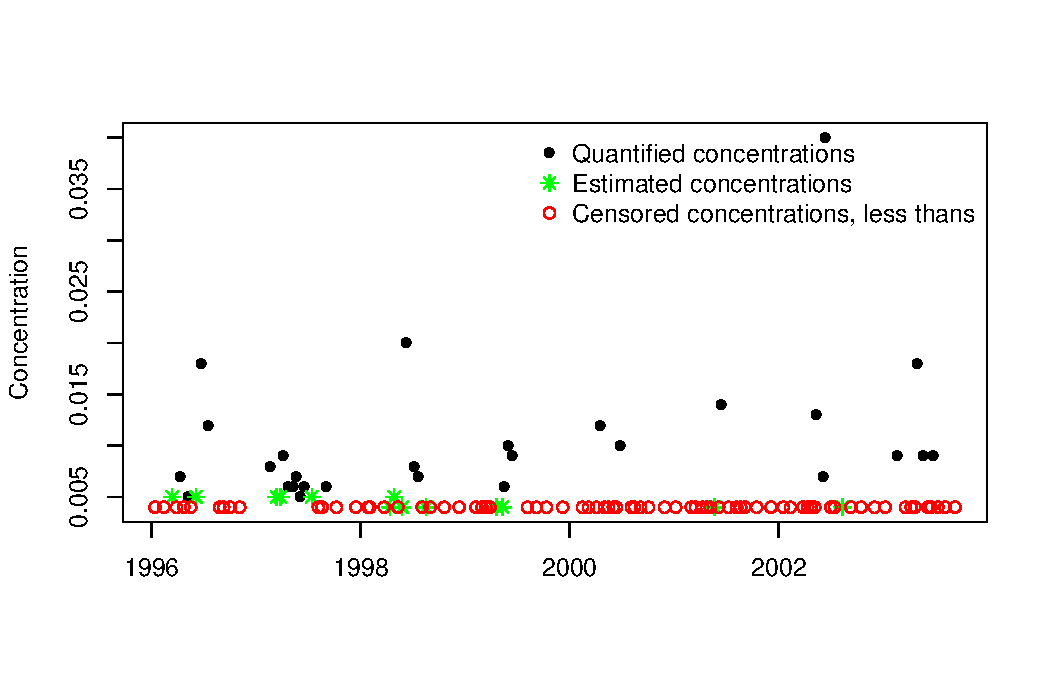
\includegraphics{vignette-002}
\end{figure}

\begin{figure}[H]
\centering
%\setkeys{Gin}{width=1.45\textwidth}
\begin{Schunk}
\begin{Sinput}
> # scatter plot with many additional plotting arguments
> # these options provide a plot closer to the plotting standards
> # of the U.S. Geological Survey, however, these plots may not 
> # meet all U.S. Geological Survey publication requirements
> par(las=1, tcl=0.5)
> cenScatPlot(qwMoRivOmaha, pname="04035", 
+                        site="06610000 Missouri River at Omaha, Nebr.",
+                        ylabel="Simazine concentration, in micrograms per liter",
+                        legcex=0.7, qwcols=c("R", "P"), ylim=c(0,0.1), yaxs="i", 
+                        cex.lab=0.9, cex.axis=0.9, xlim=c(as.Date("1996-01-01"), 
+                        as.Date("2004-01-01")), xaxs="i", xaxt="n")
> axdates <- c("1996-01-01", "1998-01-01", "2000-01-01", 
+                        "2002-01-01", "2004-01-01")
> axis(1, as.Date(axdates), 
+                        labels=c("1996", "1998", "2000", "2002", "2004"), cex.axis=0.9)
\end{Sinput}
\end{Schunk}
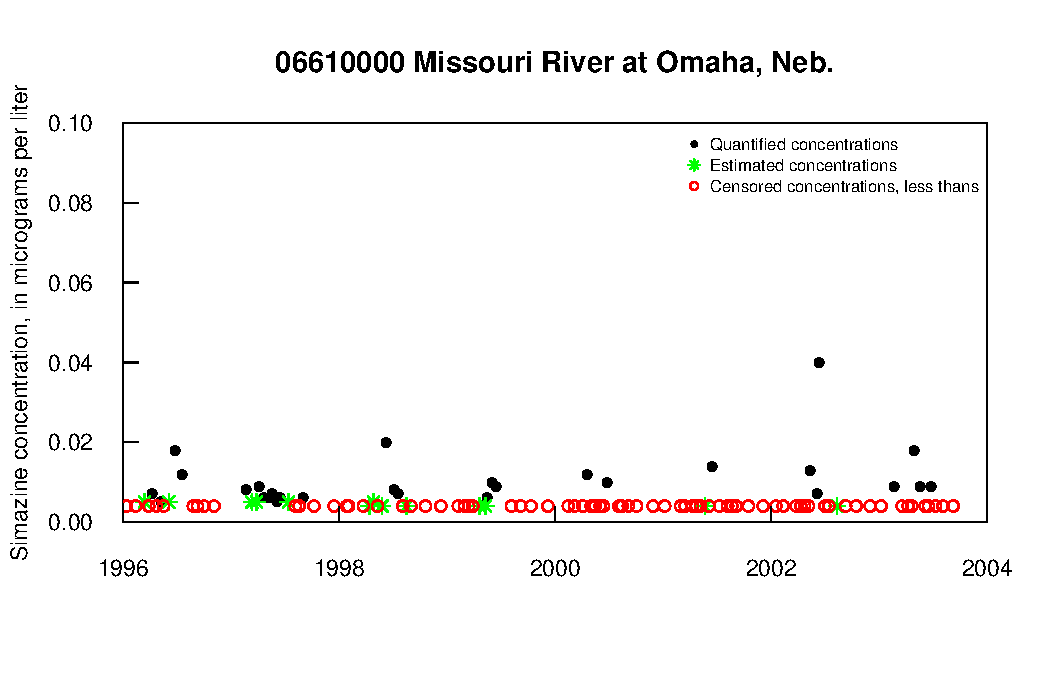
\includegraphics{vignette-003}
\end{figure}

\begin{figure}[H]
\centering
%\setkeys{Gin}{width=1.45\textwidth}
\begin{Schunk}
\begin{Sinput}
> # simple box plots of water-quality concentrations
> rosBoxPlot(qwMoRivOmaha, qwcols=c("R", "P"))
\end{Sinput}
\end{Schunk}
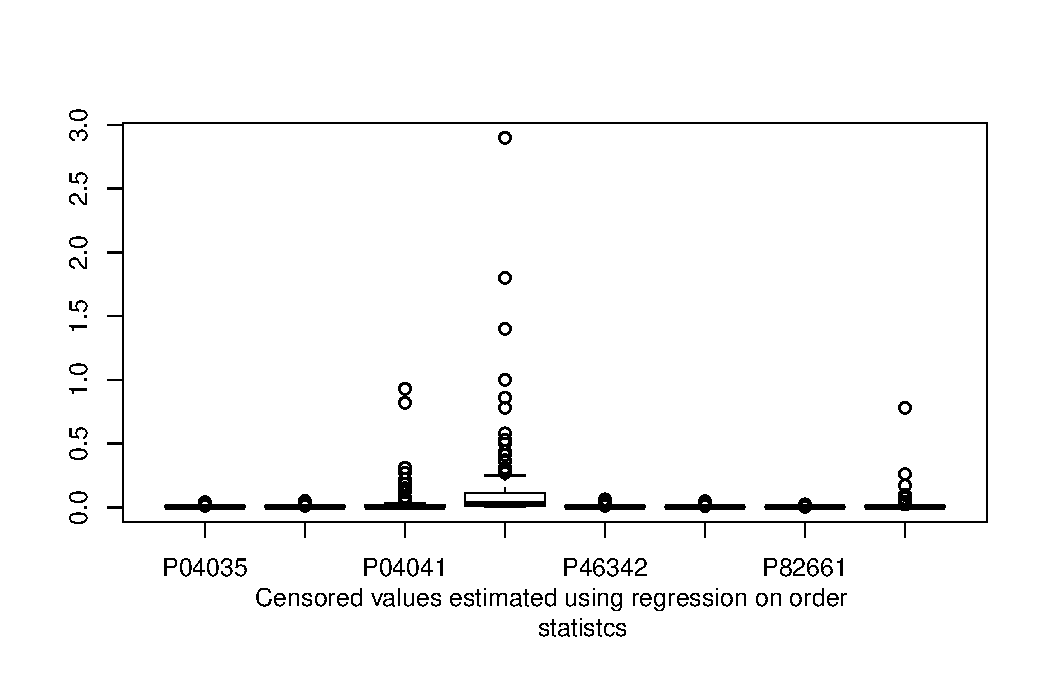
\includegraphics{vignette-004}
\end{figure}

\begin{figure}[H]
\centering
%\setkeys{Gin}{width=1.45\textwidth}
\begin{Schunk}
\begin{Sinput}
> # same boxplot function with many additional plotting arguments
> rosBoxPlot(qwMoRivOmaha, site="06610000 Missouri River at Omaha, Nebr.",
+                      log="y", yaxt="n", ylim=c(0.000001, 10), qwcols=c("R", "P"), 
+                      ylab=c("Concentration, micrograms per liter"), col="skyblue1",
+                      cex.axis=0.7, cex.sub=0.8, 
+                      par(tcl=0.5, las=1, yaxs="i", mgp=c(3,0.5,0), mar=c(5,5,2,2), 
+                      cex.main=0.9))
> axis(2, at=c(0.000001, 0.00001, 0.0001, 0.001, 0.01, 0.1, 1, 10),
+ labels=c("0.000001", "0.00001", "0.0001", "0.001", "0.01",
+ "0.1", "1", "10"), cex.axis=0.7)
\end{Sinput}
\end{Schunk}
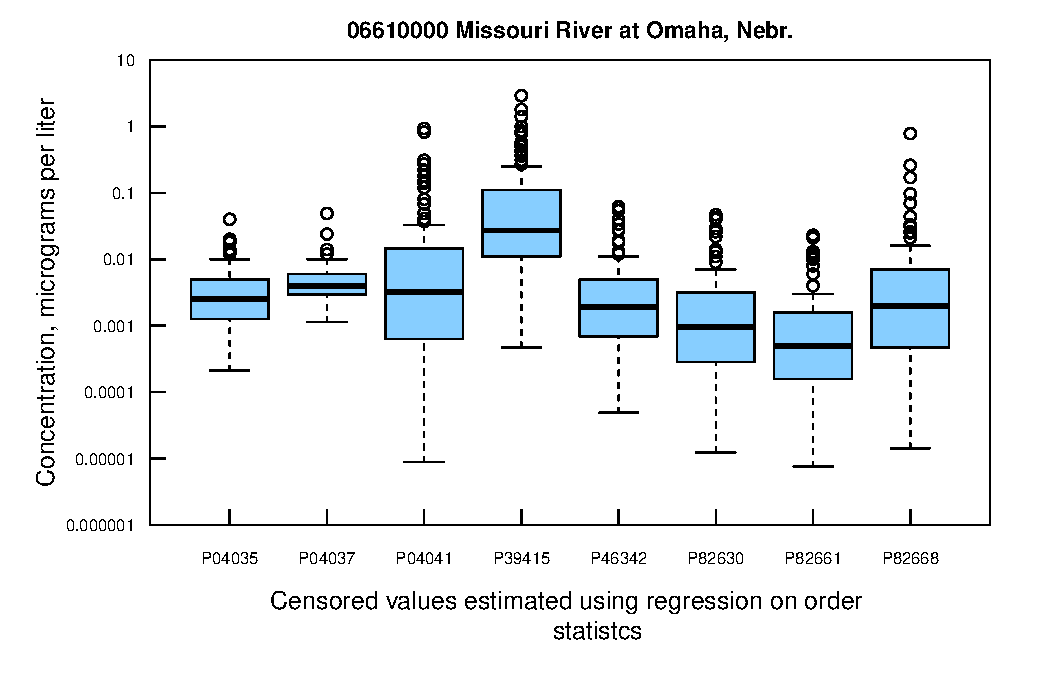
\includegraphics{vignette-005}
\end{figure}

The second data set needed is the one containing the continuous ancillary data for building the model that describes pesticide concentrations.  
\vspace{5 mm}

\begin{Schunk}
\begin{Sinput}
> data(swData)
> # show last few rows of water-quality data for Missouri River at Omaha, Nebr.
> tail(cqwMoRivOmaha)
\end{Sinput}
\begin{Soutput}
        staid      dates dflow     flowa30      flowa1 dsed
2917 06610000 2003-09-25 29200 -0.09433312 -0.00527612  176
2918 06610000 2003-09-26 28800 -0.09268448 -0.01291513  177
2919 06610000 2003-09-27 28700 -0.09102975 -0.01608045  181
2920 06610000 2003-09-28 28700 -0.08926147 -0.01784872  184
2921 06610000 2003-09-29 28600 -0.08754373 -0.02108233  189
2922 06610000 2003-09-30 28700 -0.08577546 -0.02133474  201
         seda30       seda1
2917 -0.1546322 -0.10766231
2918 -0.1566163 -0.10321762
2919 -0.1579888 -0.09213983
2920 -0.1588294 -0.08416002
2921 -0.1586754 -0.07267005
2922 -0.1569162 -0.04769499
\end{Soutput}
\begin{Sinput}
> # get a description of the data including definitions of the columns
> # by viewing the help documentation
> ?cqwMoRivOmaha
\end{Sinput}
\end{Schunk}
\vspace{5 mm}

In this case, the continuous ancillary data includes daily streamflow (dflow) and daily sediment concentration (dsed), as well as the 30-day and 1-day streamflow (flowa30 and flowa1) and sediment (seda30 and seda1) anomalies.  [The anomalies were calculated using the \textbf{waterData} package for R (Ryberg and Vecchia, 2012).]

In order to build a model using one or more of these ancillary variables as explanatory variables for pesticide concentration, the continuous ancillary variables need to be associated with the water-quality samples.  The function \textit{combineData} will combine water-quality sample data and continuous (daily) ancillary variables and drop unnecessary columns.  One needs to specify the water-quality sample data, the continuous ancillary data, and the columns representing the station identifier (staid), the sample date, the qualification code (<, E) columns, and the concentration columns as shown in the following code.  See Oblinger Childress (1999) for an explanation of the qualification codes used by the U.S. Geological Survey.
\vspace{5 mm}

\begin{Schunk}
\begin{Sinput}
> data(swData)
> MoRivOmaha<-combineData(qwdat=qwMoRivOmaha, cqwdat=cqwMoRivOmaha,
+ qwcols=c("staid", "dates", "R", "P"))
> # view combined data set
> head(MoRivOmaha)
\end{Sinput}
\begin{Soutput}
     staid      dates R04035 P04035 R04037 P04037 R04041 P04041
1 06610000 1996-01-13      <  0.004      _  0.024      <  0.008
2 06610000 1996-02-13      <  0.004      E  0.005      <  0.008
3 06610000 1996-03-13      E  0.005      E  0.004      <  0.008
4 06610000 1996-03-28      <  0.004      E  0.005      _  0.009
5 06610000 1996-04-09      _  0.007      E  0.006      _  0.014
6 06610000 1996-04-23      <  0.004      <  0.004      _  0.012
  R39415 P39415 R46342 P46342 R82630 P82630 R82661 P82661 R82668
1      _  0.006      <  0.003      _  0.029      <  0.003      _
2      _  0.200      <  0.003      <  0.007      <  0.003      _
3      _  0.026      <  0.003      <  0.007      <  0.003      E
4      _  0.026      <  0.003      <  0.007      <  0.003      _
5      _  0.075      E  0.003      <  0.007      <  0.003      _
6      _  0.040      <  0.003      <  0.007      <  0.003      <
  P82668 dflow      flowa30       flowa1 dsed      seda30
1  0.008 25800 -0.111771936 -0.041600453  255  0.04313266
2  0.007 30500 -0.155914620  0.075222364  312  0.02706313
3  0.004 32600 -0.043752697 -0.008021798  236 -0.02856792
4  0.008 42400 -0.004315925  0.066689687  609  0.01503934
5  0.009 50300  0.073100169  0.063475721  528  0.13734452
6  0.002 48800  0.126711034 -0.003283307  368  0.23175763
        seda1
1 -0.14439969
2 -0.04071575
3 -0.10632729
4  0.26177074
5  0.07748219
6 -0.17371703
\end{Soutput}
\end{Schunk}

\section{Fitting the seawaveQ Model}

One can now fit the seawaveQ model using the data explored and combined in the previous code examples.  The following code fits three different seawaveQ models (with differing continuous ancillary variables) for two pesticides in the data set.  The pesticides are 04035, simazine, and 04041, cyanazine.  See the help documentation for further information about the function arguments shown and additional arguments.
\vspace{5 mm}

\begin{Schunk}
\begin{Sinput}
> data(swData)
> # associate continuous water-quality data with each sample
> # combineData does this for you
> modMoRivOmaha<-combineData(qwdat=qwMoRivOmaha, cqwdat=cqwMoRivOmaha)
> # then fit model(s)
> myfit1 <- fitswavecav(cdat=modMoRivOmaha, cavdat=cqwMoRivOmaha,
+ tanm="myfit1", pnames=c("04035", "04041"), yrstart=1995,
+ yrend=2003, tndbeg=1995, tndend=2003, iwcav=c("flowa30", "flowa1"),
+ dcol="dates", qwcols=c("R","P"))
> myfit2 <- fitswavecav(cdat=modMoRivOmaha, cavdat=cqwMoRivOmaha,
+ tanm="myfit2", pnames=c("04035", "04041"), yrstart=1995,
+ yrend=2003, tndbeg=1995, tndend=2003, iwcav=c("seda30", "seda1"),
+ dcol="dates", qwcols=c("R","P"))
> myfit3 <- fitswavecav(cdat=modMoRivOmaha, cavdat=cqwMoRivOmaha,
+ tanm="myfit3", pnames=c("04035", "04041"), yrstart=1995,
+ yrend=2003, tndbeg=1995, tndend=2003, iwcav=c("flowa30", "flowa1",
+ "seda30", "seda1"), dcol="dates", qwcols=c("R","P"))
\end{Sinput}
\end{Schunk}

\section{Model Output}
The model fitting process finds the best pulse input function and model half-life for the concentration data and uses survival regression to fit a regression model.  Three types of output are provided: (1) a list, the first element being a data frame with information about the model and its parameters, the second element being the survival regression summary, the third element the observed concentration (censored and uncensored), the fourth element the concentrations predicted by the model, and the fifth element the summary statistics for the predicted concentrations; (2) text files showing a summary of the survival regression results, like the second element of the list, but with  additional measures of model quality and information about the R session; and (3) a pdf file of plots showing the model, trend, and diagnostic plots.  The data frame results for the three models for simazine and cyanazine are shown below.
\vspace{5 mm}

\begin{Schunk}
\begin{Sinput}
> # get the first element of the list for each model/constituent combination
> # the data frame with information about each model/constituent combination
> myfit1[[1]]
\end{Sinput}
\begin{Soutput}
  pname mclass jmod hlife   cmaxt     scl    loglik     cint
1 04035      1    3     1 0.48087 0.27216 -32.82218 -2.49433
2 04041      1    4     3 0.48087 0.42843 -43.90813 -2.27666
    cwave     ctnd cflowa30 cflowa1   seint  sewave   setnd
1 0.55360 -0.02850  0.05509 2.09772 0.04908 0.11183 0.02191
2 2.16327 -0.25063  0.00587 2.95546 0.08622 0.26127 0.03775
  seflowa30 seflowa1
1   0.30734  0.46967
2   0.52071  0.78638
\end{Soutput}
\begin{Sinput}
> myfit2[[1]]
\end{Sinput}
\begin{Soutput}
  pname mclass jmod hlife   cmaxt     scl    loglik     cint
1 04035      1    5     3 0.48087 0.24680 -24.33186 -2.68415
2 04041      1    3     2 0.48087 0.41225 -40.46237 -2.13390
    cwave     ctnd cseda30  cseda1   seint  sewave   setnd
1 0.79622 -0.02478 0.25178 0.59654 0.06853 0.18670 0.01637
2 1.57758 -0.22234 1.14307 0.62894 0.07579 0.19086 0.02996
  seseda30 seseda1
1  0.17377 0.10251
2  0.29031 0.18224
\end{Soutput}
\begin{Sinput}
> myfit3[[1]]
\end{Sinput}
\begin{Soutput}
  pname mclass jmod hlife   cmaxt     scl    loglik     cint
1 04035      1    5     3 0.48087 0.24625 -23.83840 -2.67858
2 04041      1    3     2 0.48087 0.39523 -38.65962 -2.08402
    cwave     ctnd cflowa30  cflowa1 cseda30  cseda1   seint
1 0.76537 -0.01883  0.17756 -0.36824 0.22666 0.66734 0.06725
2 1.70493 -0.24244 -0.57741  1.53888 1.04420 0.29466 0.07942
   sewave   setnd seflowa30 seflowa1 seseda30 seseda1
1 0.18450 0.01991   0.30663  0.64400  0.20480 0.15247
2 0.20191 0.03459   0.50123  1.12286  0.31298 0.27108
\end{Soutput}
\begin{Sinput}
> # get the second element of the list for each model/constituent combination
> # the survival regression summary for each model/constituent combination
> myfit1[[2]]
\end{Sinput}
\begin{Soutput}
[[1]]

Call:
survreg(formula = Surv(time = clogtmp, time2 = indcen, type = "left") ~ 
    xxxmat - 1, dist = "gaussian")
                Value Std. Error       z        p
xxxmatintcpt  -2.4943     0.0491 -50.826 0.00e+00
xxxmatwavest   0.5536     0.1118   4.950 7.41e-07
xxxmattndlin  -0.0285     0.0219  -1.301 1.93e-01
xxxmatflowa30  0.0551     0.3073   0.179 8.58e-01
xxxmatflowa1   2.0977     0.4697   4.466 7.96e-06
Log(scale)    -1.3013     0.1205 -10.797 3.57e-27

Scale= 0.272 

Gaussian distribution
Loglik(model)= -32.8   Loglik(intercept only)= -60.9
	Chisq= 56.1 on 4 degrees of freedom, p= 1.9e-11 
Number of Newton-Raphson Iterations: 5 
n= 115 


[[2]]

Call:
survreg(formula = Surv(time = clogtmp, time2 = indcen, type = "left") ~ 
    xxxmat - 1, dist = "gaussian")
                 Value Std. Error        z         p
xxxmatintcpt  -2.27666     0.0862 -26.4055 1.19e-153
xxxmatwavest   2.16327     0.2613   8.2799  1.23e-16
xxxmattndlin  -0.25063     0.0377  -6.6393  3.15e-11
xxxmatflowa30  0.00587     0.5207   0.0113  9.91e-01
xxxmatflowa1   2.95546     0.7864   3.7583  1.71e-04
Log(scale)    -0.84763     0.1038  -8.1685  3.12e-16

Scale= 0.428 

Gaussian distribution
Loglik(model)= -43.9   Loglik(intercept only)= -103.7
	Chisq= 119.63 on 4 degrees of freedom, p= 0 
Number of Newton-Raphson Iterations: 6 
n= 115 
\end{Soutput}
\begin{Sinput}
> myfit2[[2]]
\end{Sinput}
\begin{Soutput}
[[1]]

Call:
survreg(formula = Surv(time = clogtmp, time2 = indcen, type = "left") ~ 
    xxxmat - 1, dist = "gaussian")
               Value Std. Error      z        p
xxxmatintcpt -2.6841     0.0685 -39.17 0.00e+00
xxxmatwavest  0.7962     0.1867   4.26 2.00e-05
xxxmattndlin -0.0248     0.0164  -1.51 1.30e-01
xxxmatseda30  0.2518     0.1738   1.45 1.47e-01
xxxmatseda1   0.5965     0.1025   5.82 5.90e-09
Log(scale)   -1.3992     0.1184 -11.82 3.16e-32

Scale= 0.247 

Gaussian distribution
Loglik(model)= -24.3   Loglik(intercept only)= -60.9
	Chisq= 73.08 on 4 degrees of freedom, p= 5.1e-15 
Number of Newton-Raphson Iterations: 6 
n= 115 


[[2]]

Call:
survreg(formula = Surv(time = clogtmp, time2 = indcen, type = "left") ~ 
    xxxmat - 1, dist = "gaussian")
              Value Std. Error      z         p
xxxmatintcpt -2.134     0.0758 -28.15 2.10e-174
xxxmatwavest  1.578     0.1909   8.27  1.39e-16
xxxmattndlin -0.222     0.0300  -7.42  1.15e-13
xxxmatseda30  1.143     0.2903   3.94  8.24e-05
xxxmatseda1   0.629     0.1822   3.45  5.58e-04
Log(scale)   -0.886     0.1029  -8.61  7.00e-18

Scale= 0.412 

Gaussian distribution
Loglik(model)= -40.5   Loglik(intercept only)= -103.7
	Chisq= 126.52 on 4 degrees of freedom, p= 0 
Number of Newton-Raphson Iterations: 6 
n= 115 
\end{Soutput}
\begin{Sinput}
> myfit3[[2]]
\end{Sinput}
\begin{Soutput}
[[1]]

Call:
survreg(formula = Surv(time = clogtmp, time2 = indcen, type = "left") ~ 
    xxxmat - 1, dist = "gaussian")
                Value Std. Error       z        p
xxxmatintcpt  -2.6786     0.0673 -39.828 0.00e+00
xxxmatwavest   0.7654     0.1845   4.148 3.35e-05
xxxmattndlin  -0.0188     0.0199  -0.946 3.44e-01
xxxmatflowa30  0.1776     0.3066   0.579 5.63e-01
xxxmatflowa1  -0.3682     0.6440  -0.572 5.67e-01
xxxmatseda30   0.2267     0.2048   1.107 2.68e-01
xxxmatseda1    0.6673     0.1525   4.377 1.20e-05
Log(scale)    -1.4014     0.1188 -11.800 3.92e-32

Scale= 0.246 

Gaussian distribution
Loglik(model)= -23.8   Loglik(intercept only)= -60.9
	Chisq= 74.06 on 6 degrees of freedom, p= 6e-14 
Number of Newton-Raphson Iterations: 6 
n= 115 


[[2]]

Call:
survreg(formula = Surv(time = clogtmp, time2 = indcen, type = "left") ~ 
    xxxmat - 1, dist = "gaussian")
               Value Std. Error      z         p
xxxmatintcpt  -2.084     0.0794 -26.24 9.36e-152
xxxmatwavest   1.705     0.2019   8.44  3.07e-17
xxxmattndlin  -0.242     0.0346  -7.01  2.39e-12
xxxmatflowa30 -0.577     0.5012  -1.15  2.49e-01
xxxmatflowa1   1.539     1.1229   1.37  1.71e-01
xxxmatseda30   1.044     0.3130   3.34  8.49e-04
xxxmatseda1    0.295     0.2711   1.09  2.77e-01
Log(scale)    -0.928     0.1035  -8.97  3.00e-19

Scale= 0.395 

Gaussian distribution
Loglik(model)= -38.7   Loglik(intercept only)= -103.7
	Chisq= 130.12 on 6 degrees of freedom, p= 0 
Number of Newton-Raphson Iterations: 6 
n= 115 
\end{Soutput}
\begin{Sinput}
> # get the first few lines of the third element of the list
> head(myfit1[[3]])